\documentclass[12pt,a4paper]{article}
\usepackage{caption}
\usepackage{float}
\usepackage[left=2cm, right=2cm, top=2cm, bottom=2cm]{geometry}
\usepackage{graphicx}
\usepackage{subcaption}
\usepackage{xeCJK}

\captionsetup[figure]{labelformat=empty}
\subcaptionsetup[figure]{labelformat=empty}
\setCJKmainfont{新細明體}

\title{
  Quartus II Lab1 \textemdash\ Combinational Circuits\\
  \large NTU Switching Circuit and Logic Design 2023
}
\author{B12902110 呂承諺}
\date{}

\begin{document}
  \maketitle
  \section{FA: 1-bit Full Adder}
  \begin{figure}[H]
    \centering
    \begin{subcaptionblock}{0.15\linewidth}
      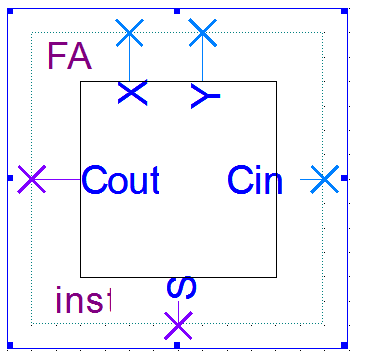
\includegraphics[width=\linewidth]{FA_bsf.png}
      \caption{FA.bsf}
    \end{subcaptionblock}
    \begin{subcaptionblock}{0.84\linewidth}
      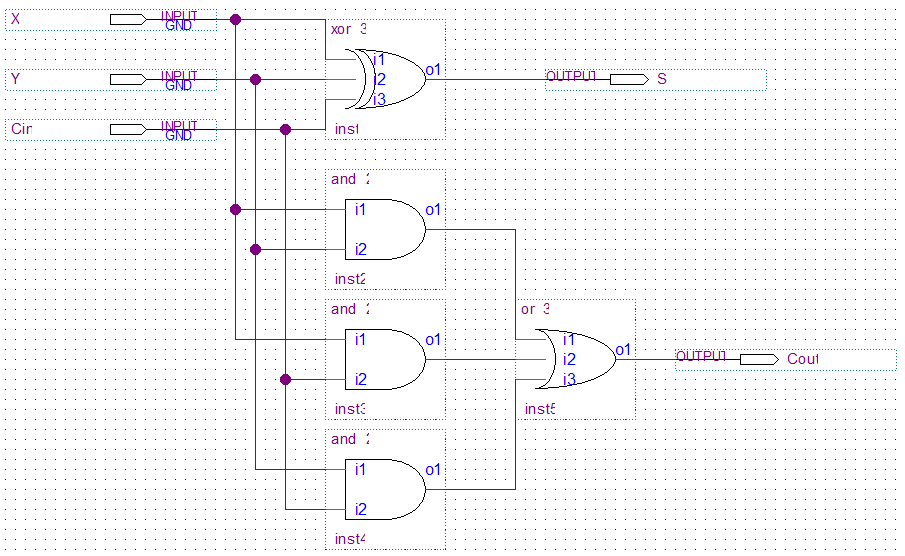
\includegraphics[width=\linewidth]{FA_bdf.png}
      \caption{FA.bdf}
    \end{subcaptionblock}
  \end{figure}

  \section{FA4: 4-bit Adder}
  \begin{figure}[H]
    \centering
    \begin{subcaptionblock}{0.15\linewidth}
      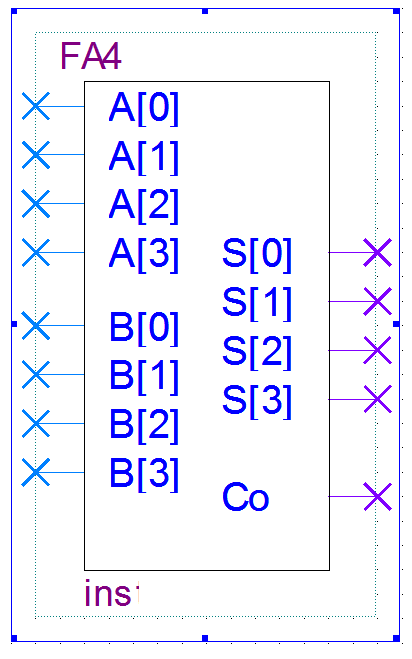
\includegraphics[width=\linewidth]{FA4_bsf.png}
      \caption{FA4.bsf}
    \end{subcaptionblock}
    \begin{subcaptionblock}{0.84\linewidth}
      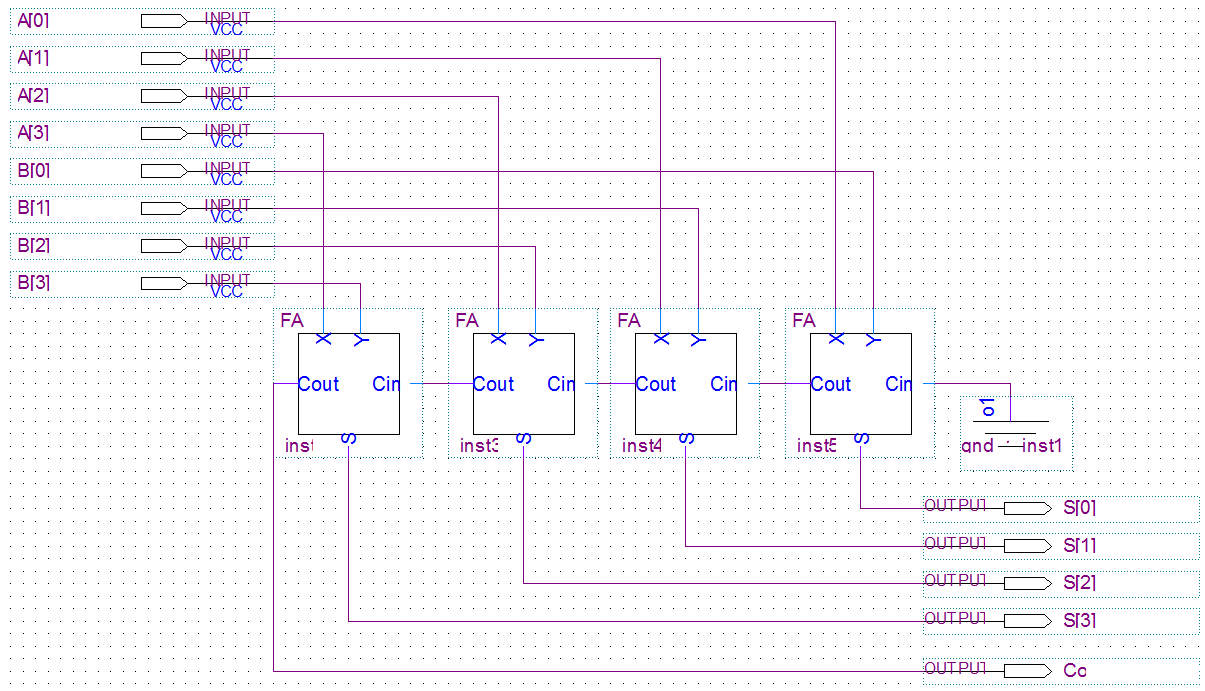
\includegraphics[width=\linewidth]{FA4_bdf.png}
      \caption{FA4.bdf}
    \end{subcaptionblock}
  \end{figure}
  \begin{figure}[H]
    \centering
    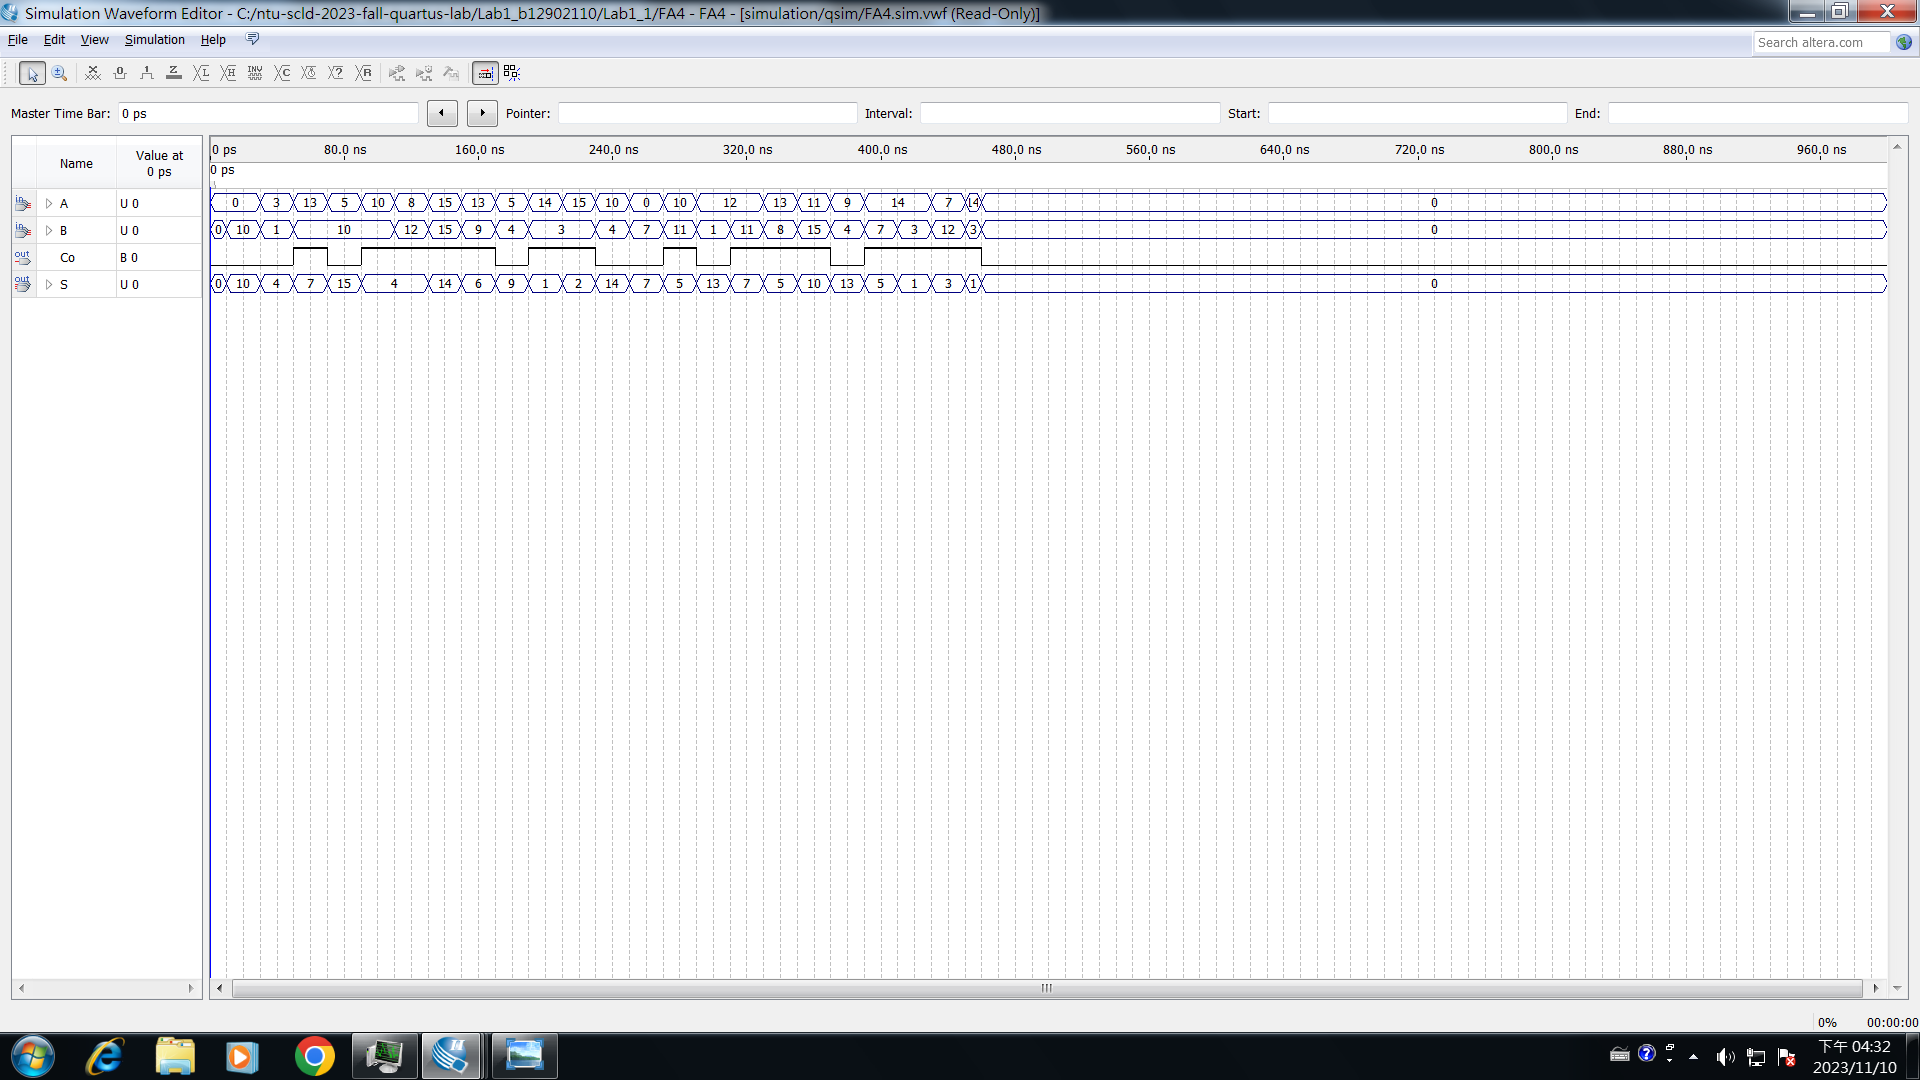
\includegraphics[width=\linewidth]{FA4_simulation.png}
    \caption{FA4 simulation}
  \end{figure}

  \section{FS: 1-bit Full Subtrator}
  \begin{figure}[H]
    \centering
    \begin{subcaptionblock}{0.15\linewidth}
      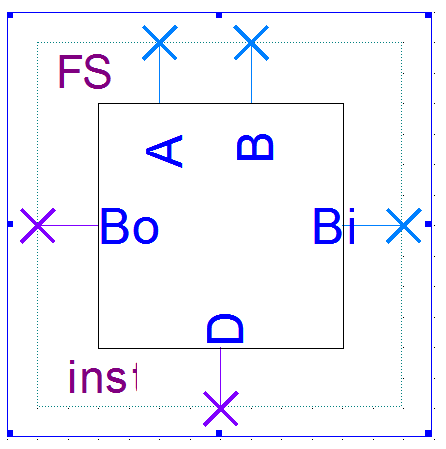
\includegraphics[width=\linewidth]{FS_bsf.png}
      \caption{FS.bsf}
    \end{subcaptionblock}
    \begin{subcaptionblock}{0.84\linewidth}
      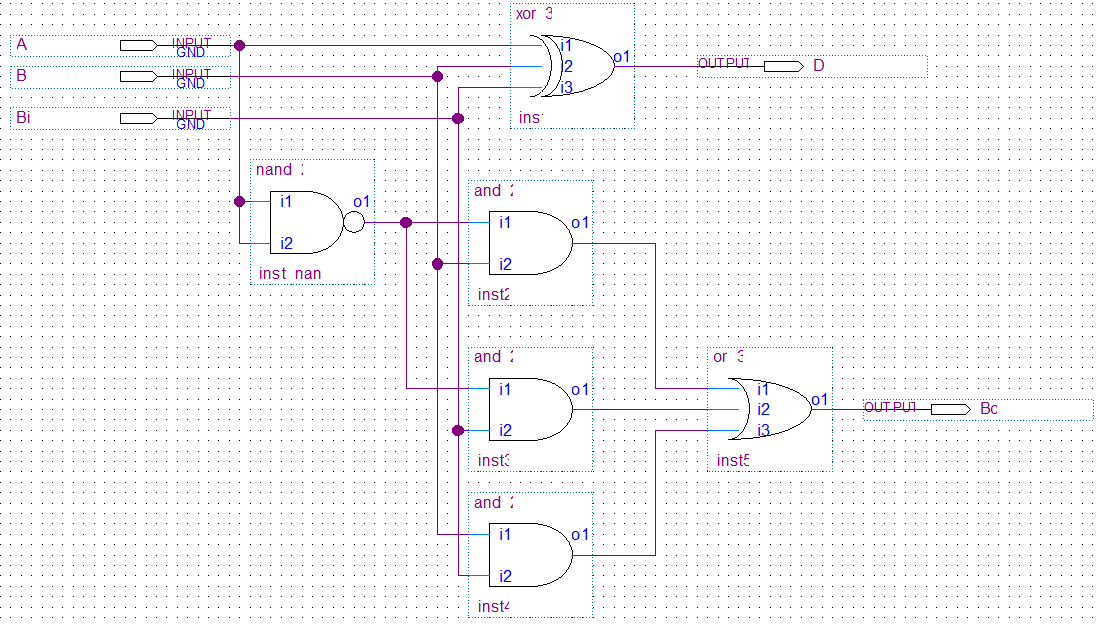
\includegraphics[width=\linewidth]{FS_bdf.png}
      \caption{FS.bdf}
    \end{subcaptionblock}
  \end{figure}

  \section{FS4: 4-bit Subtractor}
  \begin{figure}[H]
    \centering
    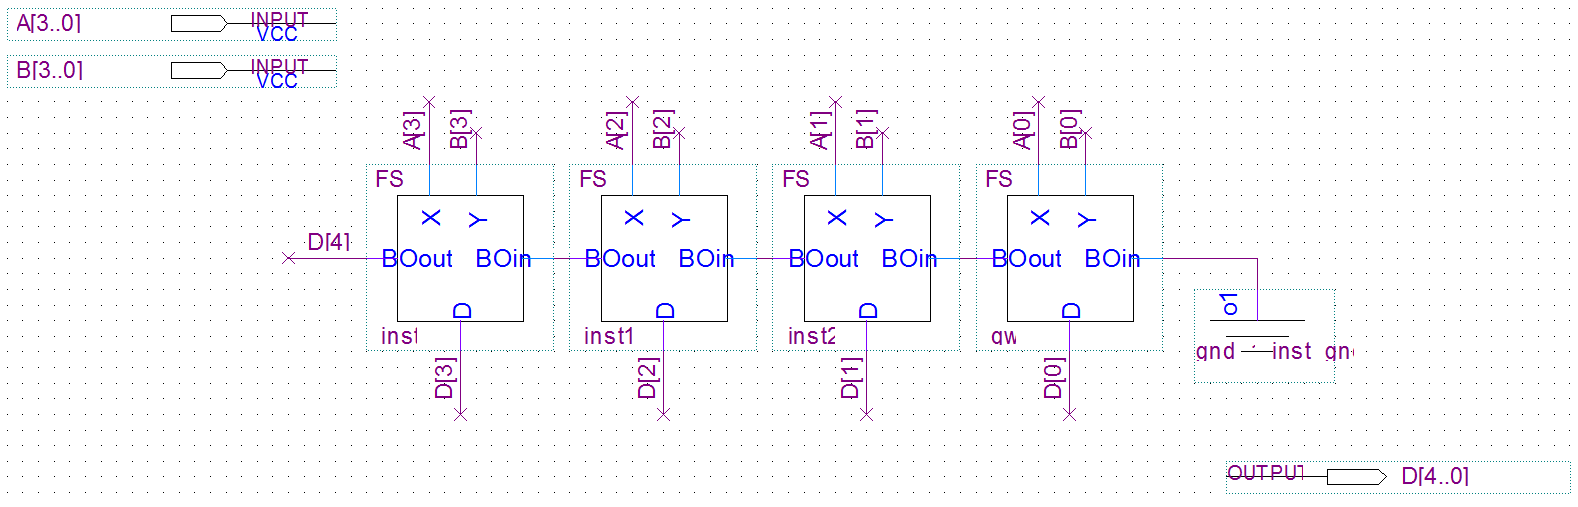
\includegraphics[width=\linewidth]{FS4_bdf.png}
    \caption{FS4.bdf}
  \end{figure}
  \begin{figure}[H]
    \centering
    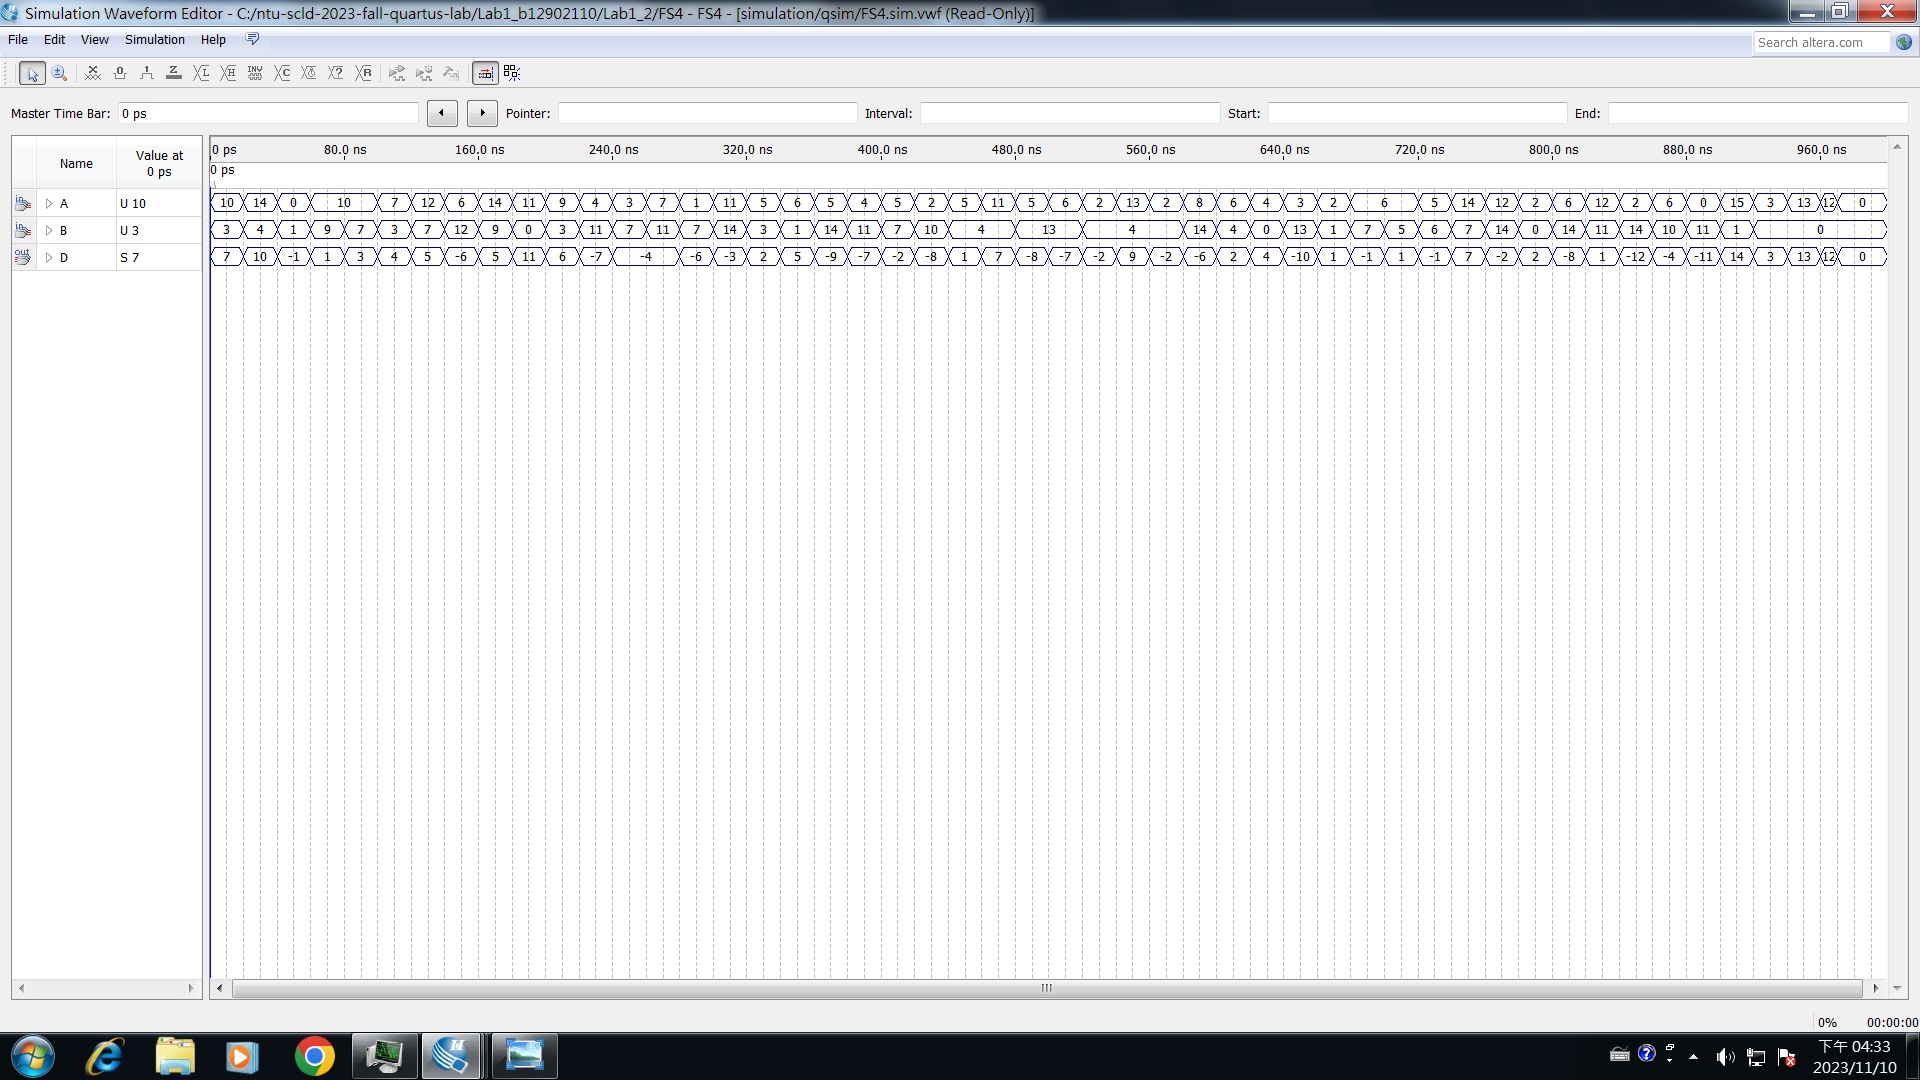
\includegraphics[width=\linewidth]{FS4_simulation.png}
    \caption{FS4 simulation}
  \end{figure}

  \section{GATE4: 4-bit Gate}
  if (G == 1) then B = A\\
  else B = 0
  \begin{figure}[H]
    \centering
    \begin{subcaptionblock}{0.15\linewidth}
        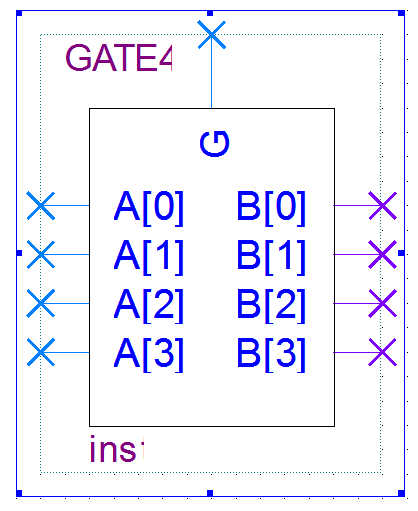
\includegraphics[width=\linewidth]{GATE4_bsf.png}
        \caption{GATE4.bsf}
    \end{subcaptionblock}
    \begin{subcaptionblock}{0.84\linewidth}
        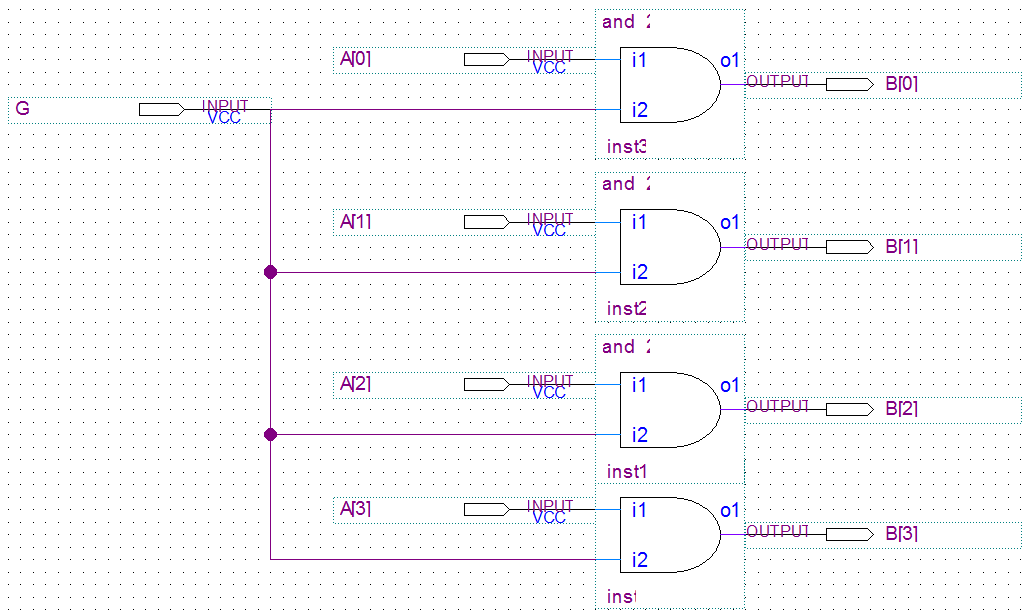
\includegraphics[width=\linewidth]{GATE4_bdf.png}
        \caption{GATE4.bdf}
    \end{subcaptionblock}
  \end{figure}

  \section{MU4: 4-bit Multiplier}
  \begin{figure}[H]
    \centering
    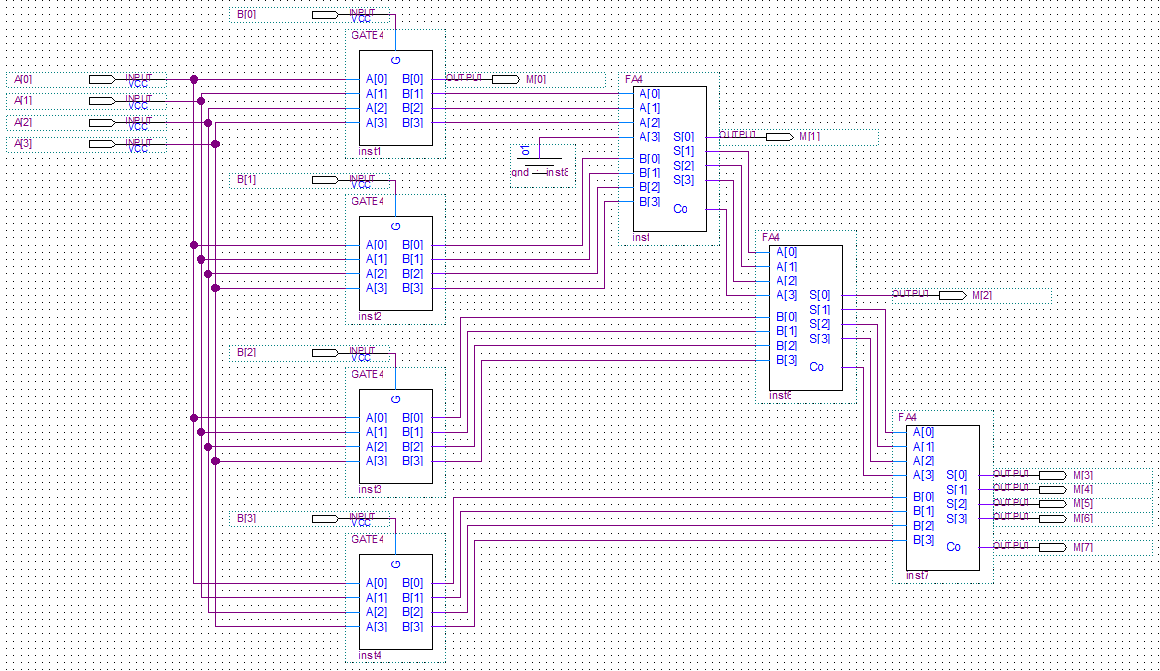
\includegraphics[width=\linewidth]{MU4_bdf.png}
    \caption{MU4.bdf}
  \end{figure}
  \begin{figure}[H]
    \centering
    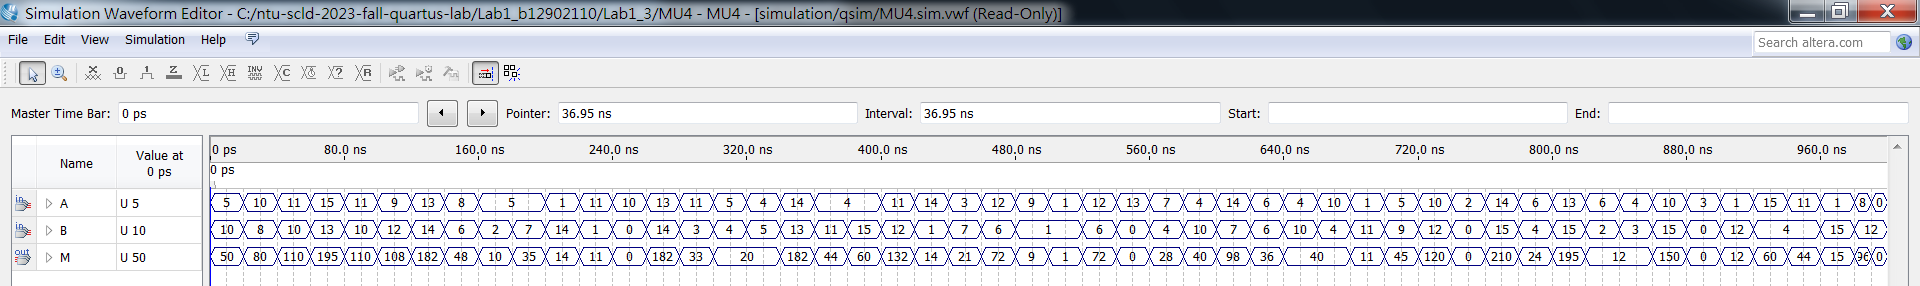
\includegraphics[width=\linewidth]{MU4_simulation.png}
    \caption{MU4 simulation}
  \end{figure}
\end{document}
